\begin{figure}[H]
    \centering
    \begin{subfigure}[b]{0.48\textwidth}
        \centering
        \begin{minipage}{0.32\textwidth}
            \centering
            \includegraphics[width=\textwidth]{figures/DRAEMweakness/structural026image.png}
        \end{minipage}
        \begin{minipage}{0.32\textwidth}
            \centering
            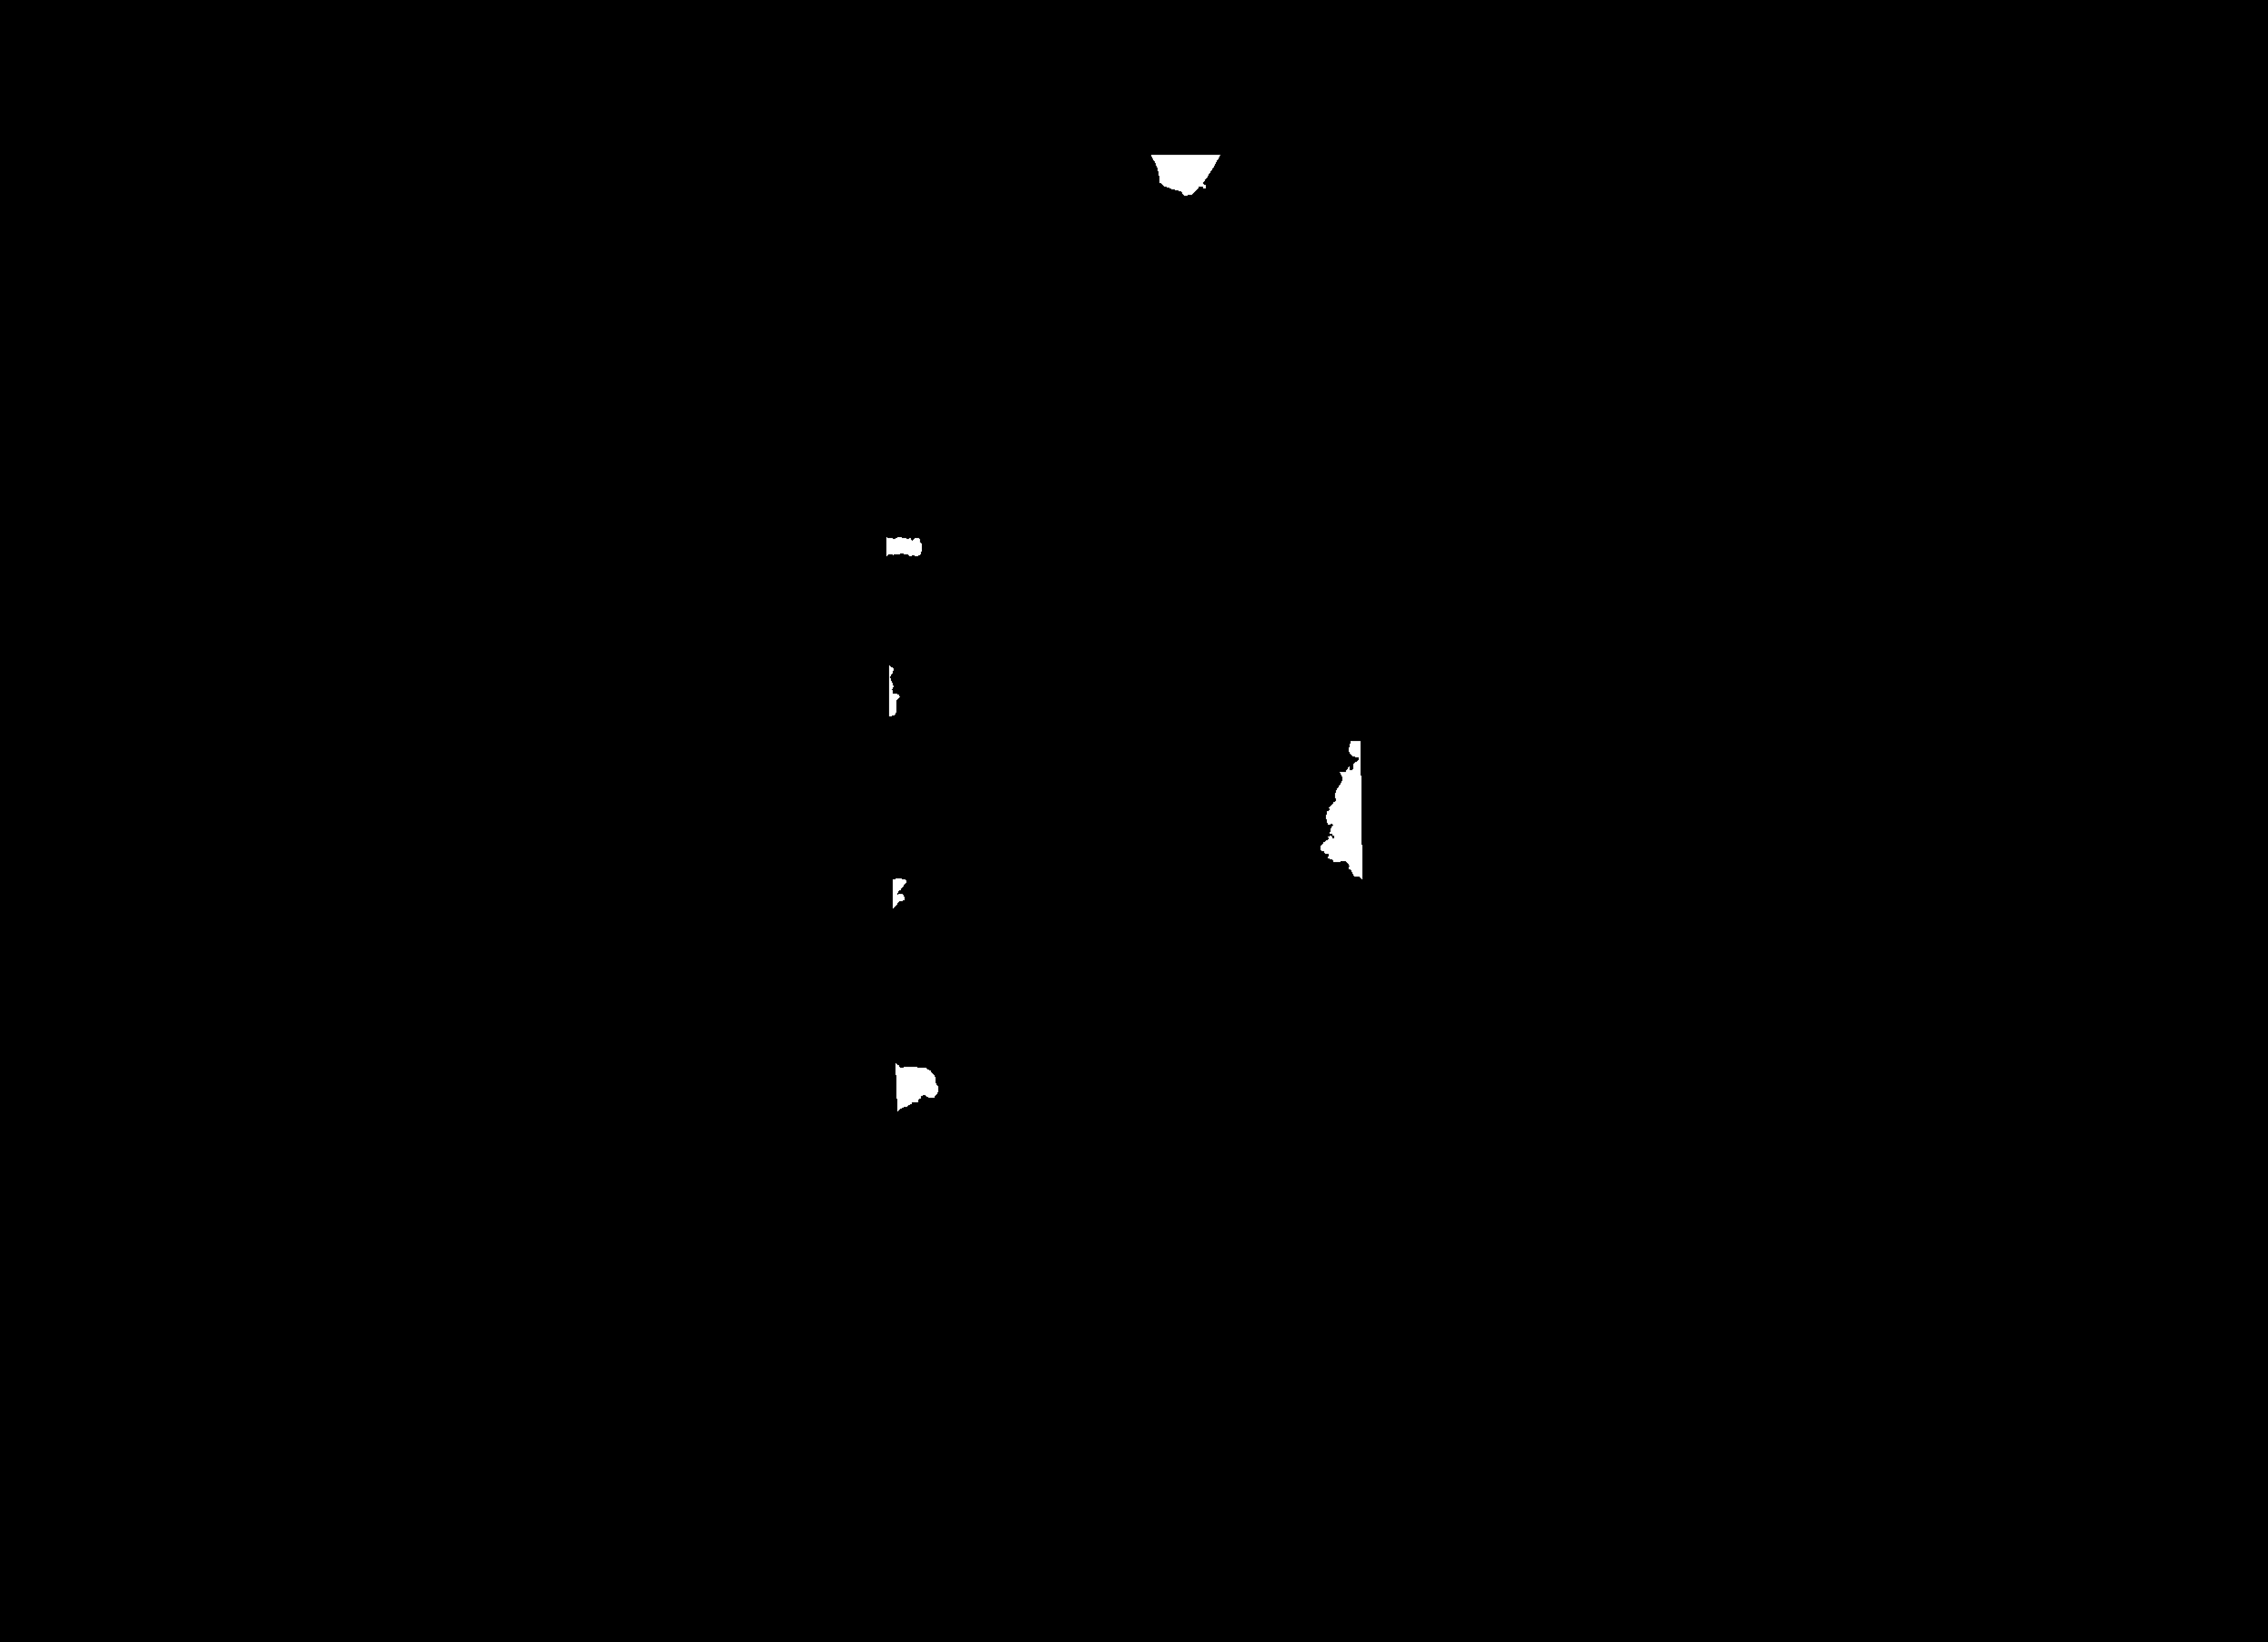
\includegraphics[width=\textwidth]{figures/DRAEMweakness/structural026mask.png}
        \end{minipage}
        \begin{minipage}{0.32\textwidth}
            \centering
            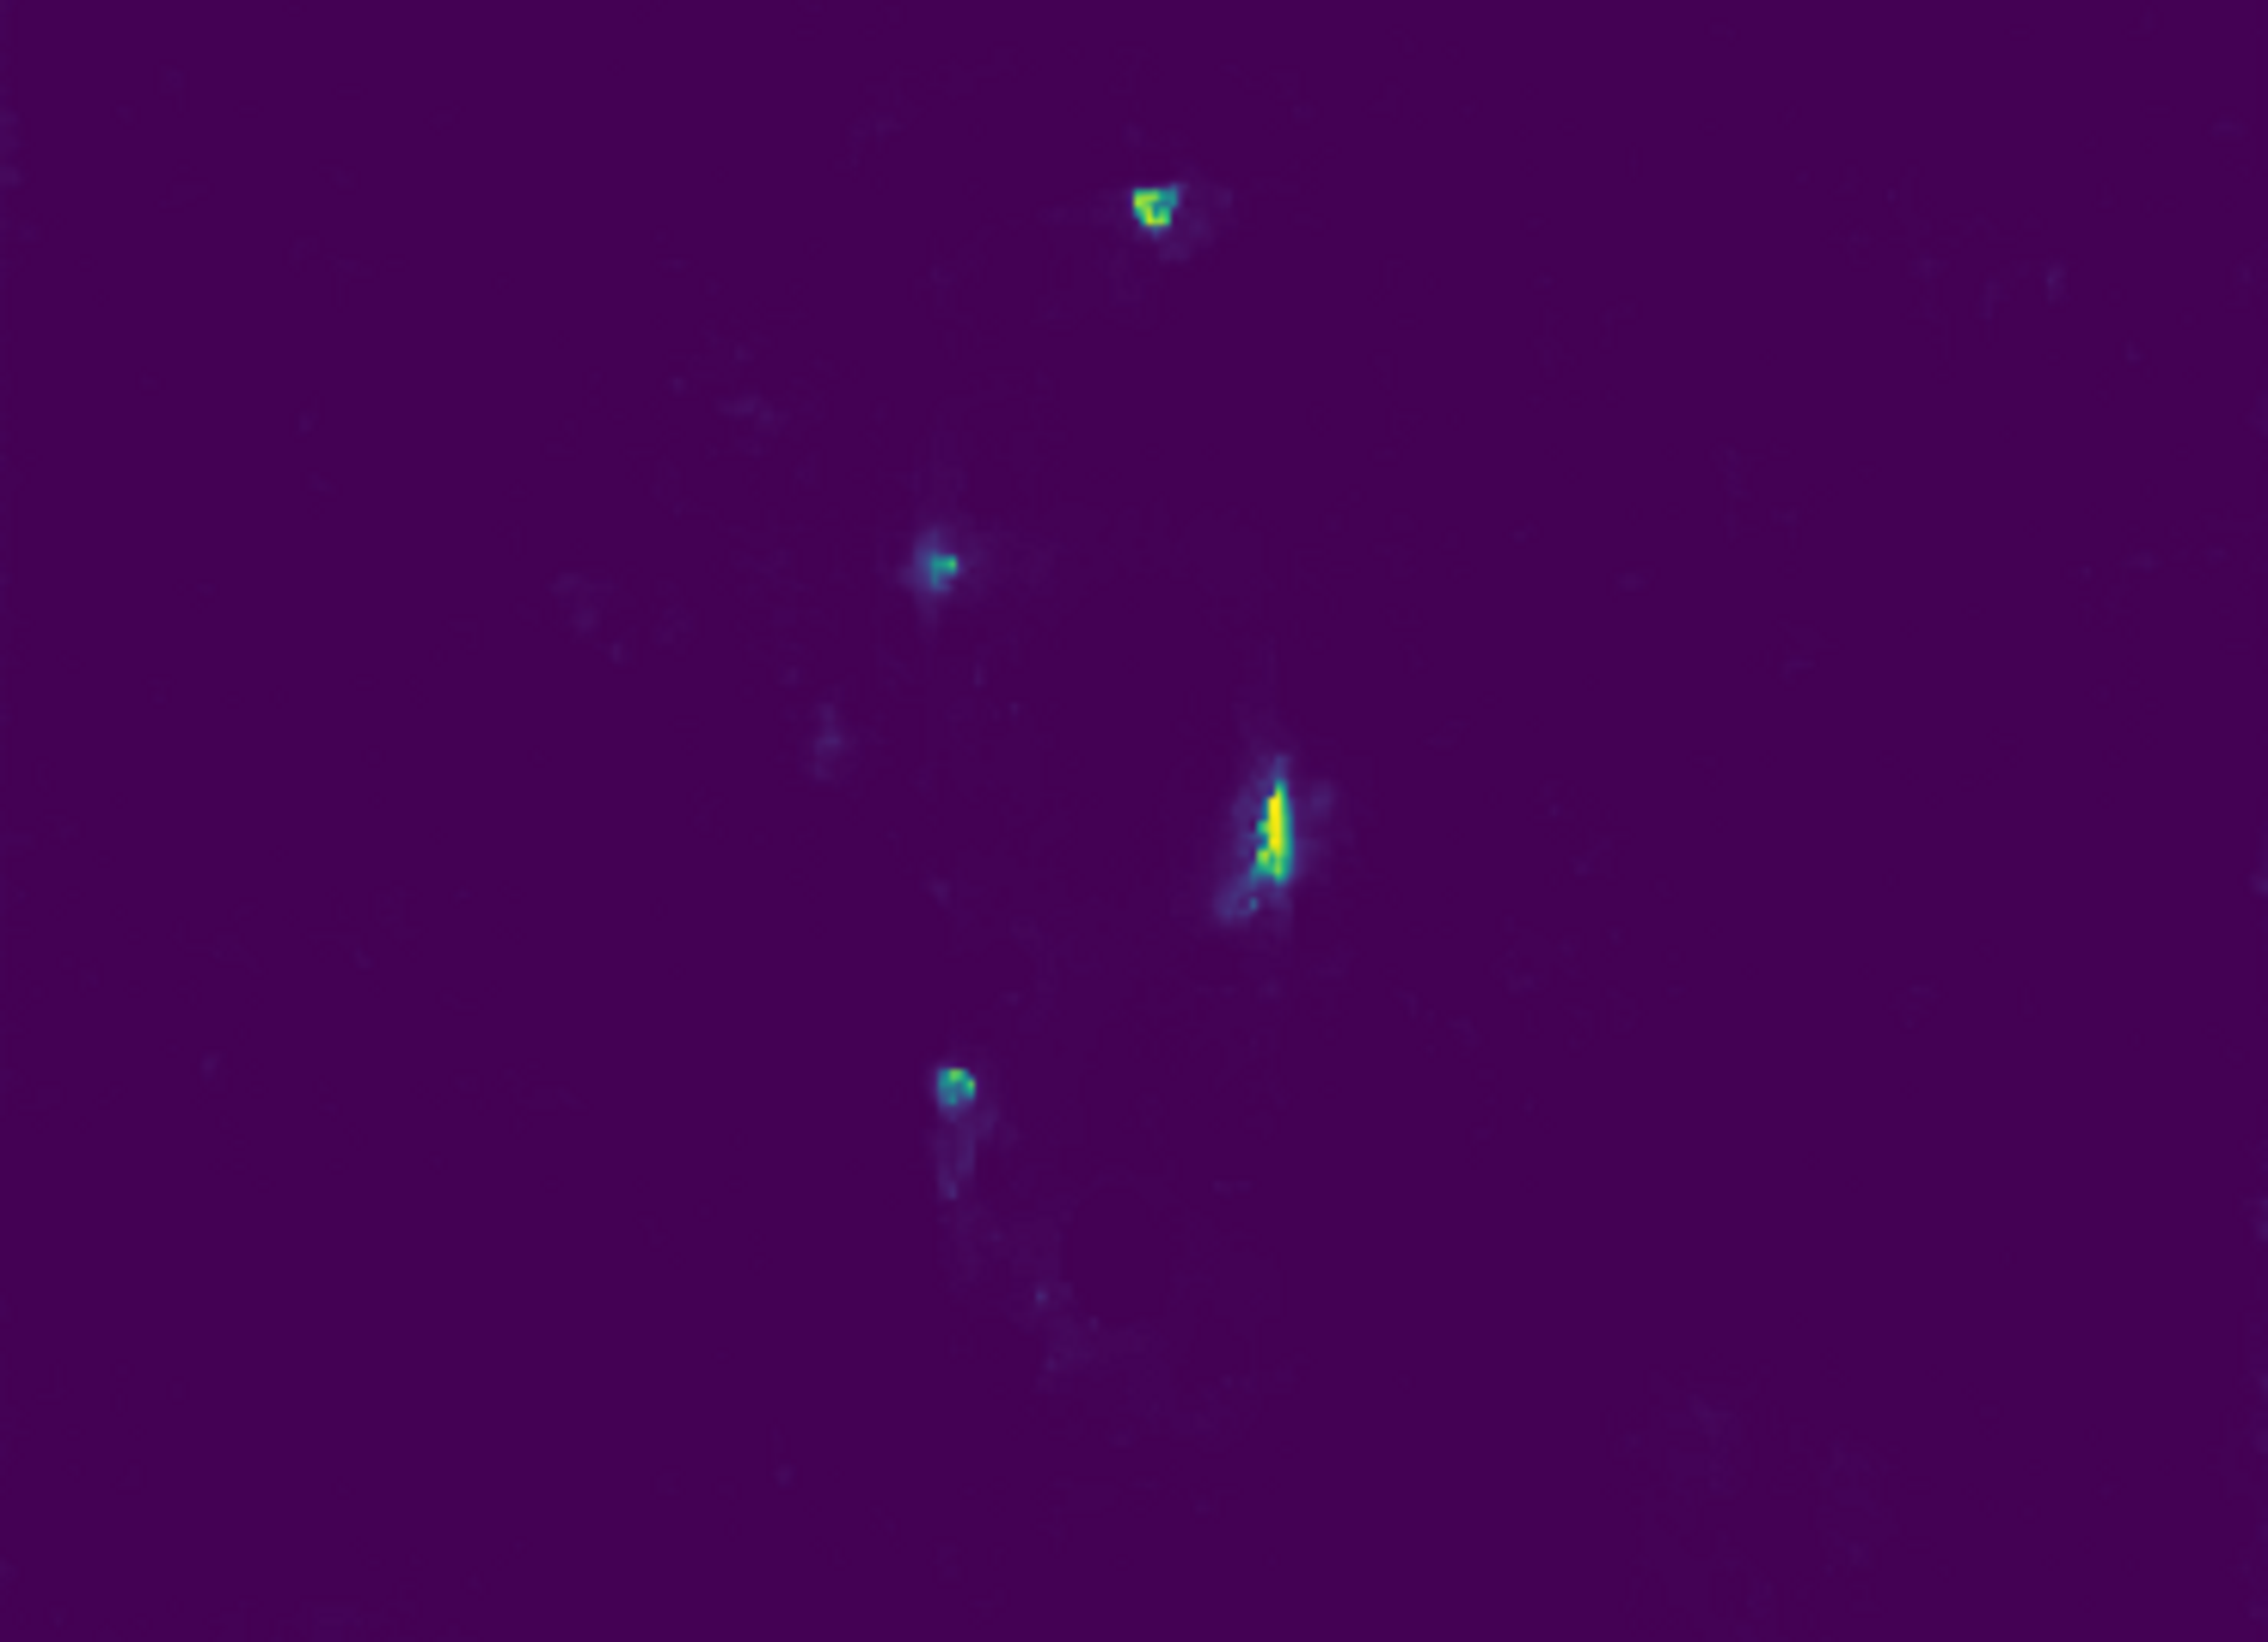
\includegraphics[width=\textwidth]{figures/DRAEMweakness/structural026segment.png}
        \end{minipage}
        \caption{Subfigure 1}
    \end{subfigure}
    \hfill
    \begin{subfigure}[b]{0.48\textwidth}
        \centering
        \begin{minipage}{0.32\textwidth}
            \centering
            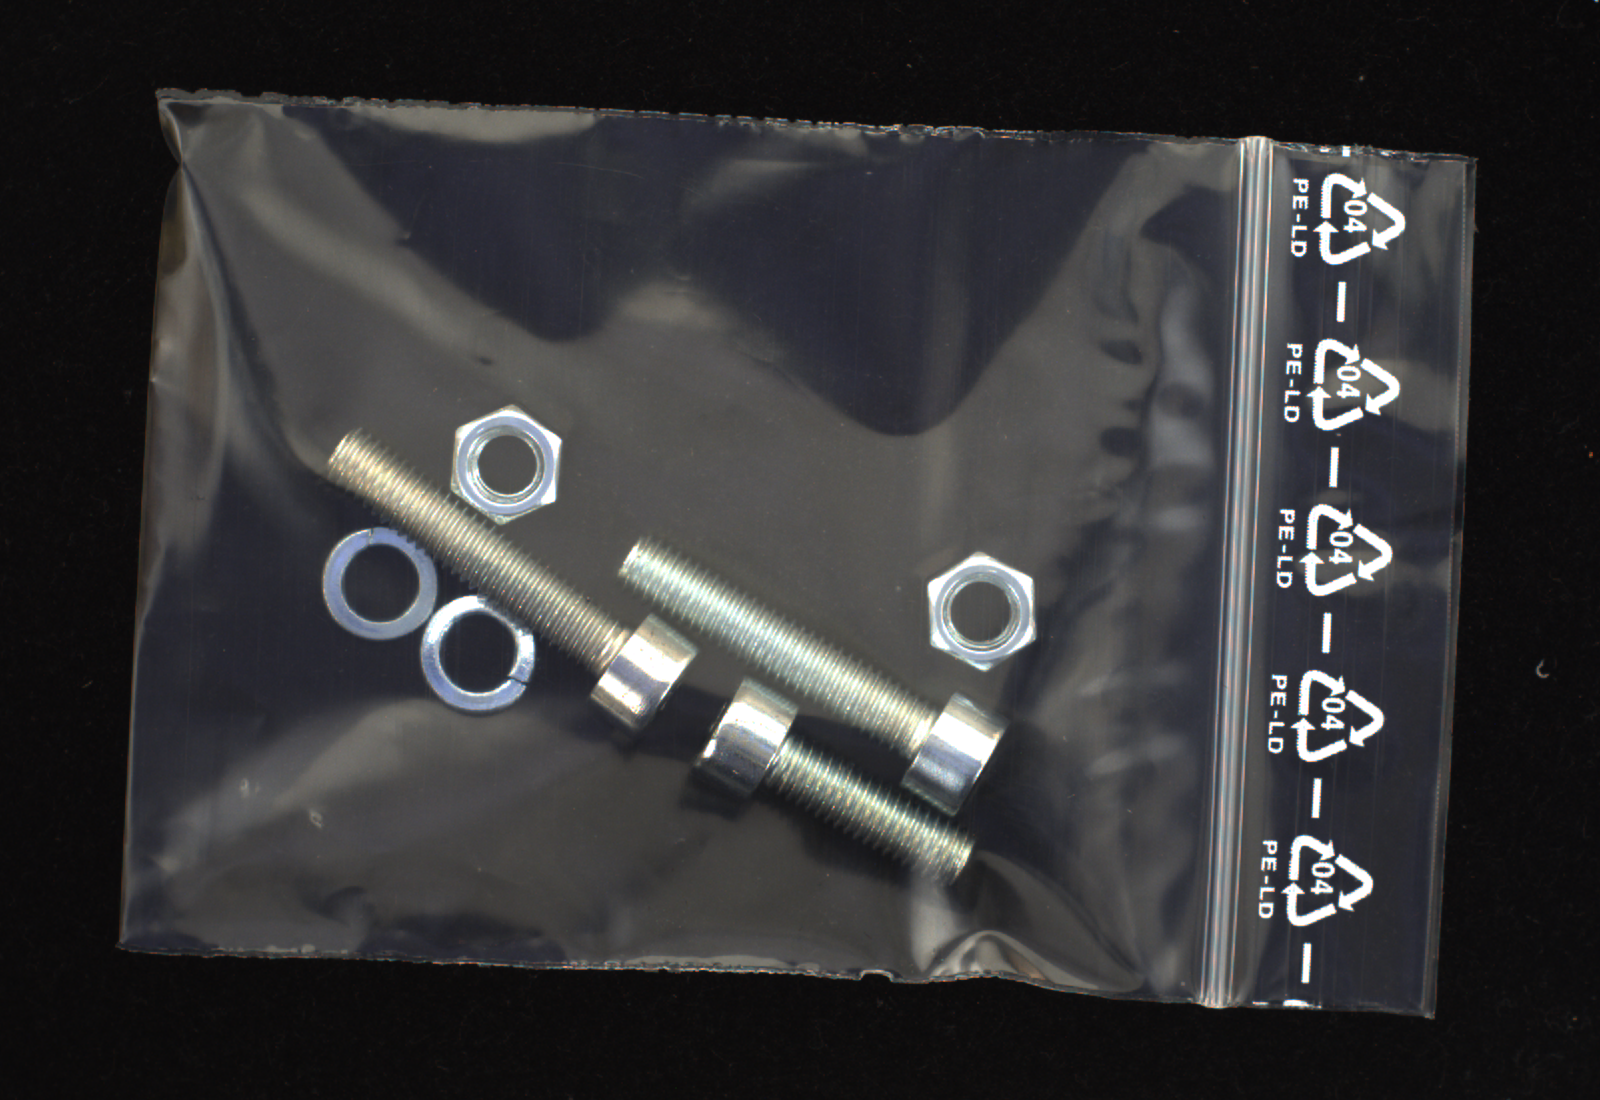
\includegraphics[width=\textwidth]{figures/DRAEMweakness/logical042image.png}
        \end{minipage}
        \begin{minipage}{0.32\textwidth}
            \centering
            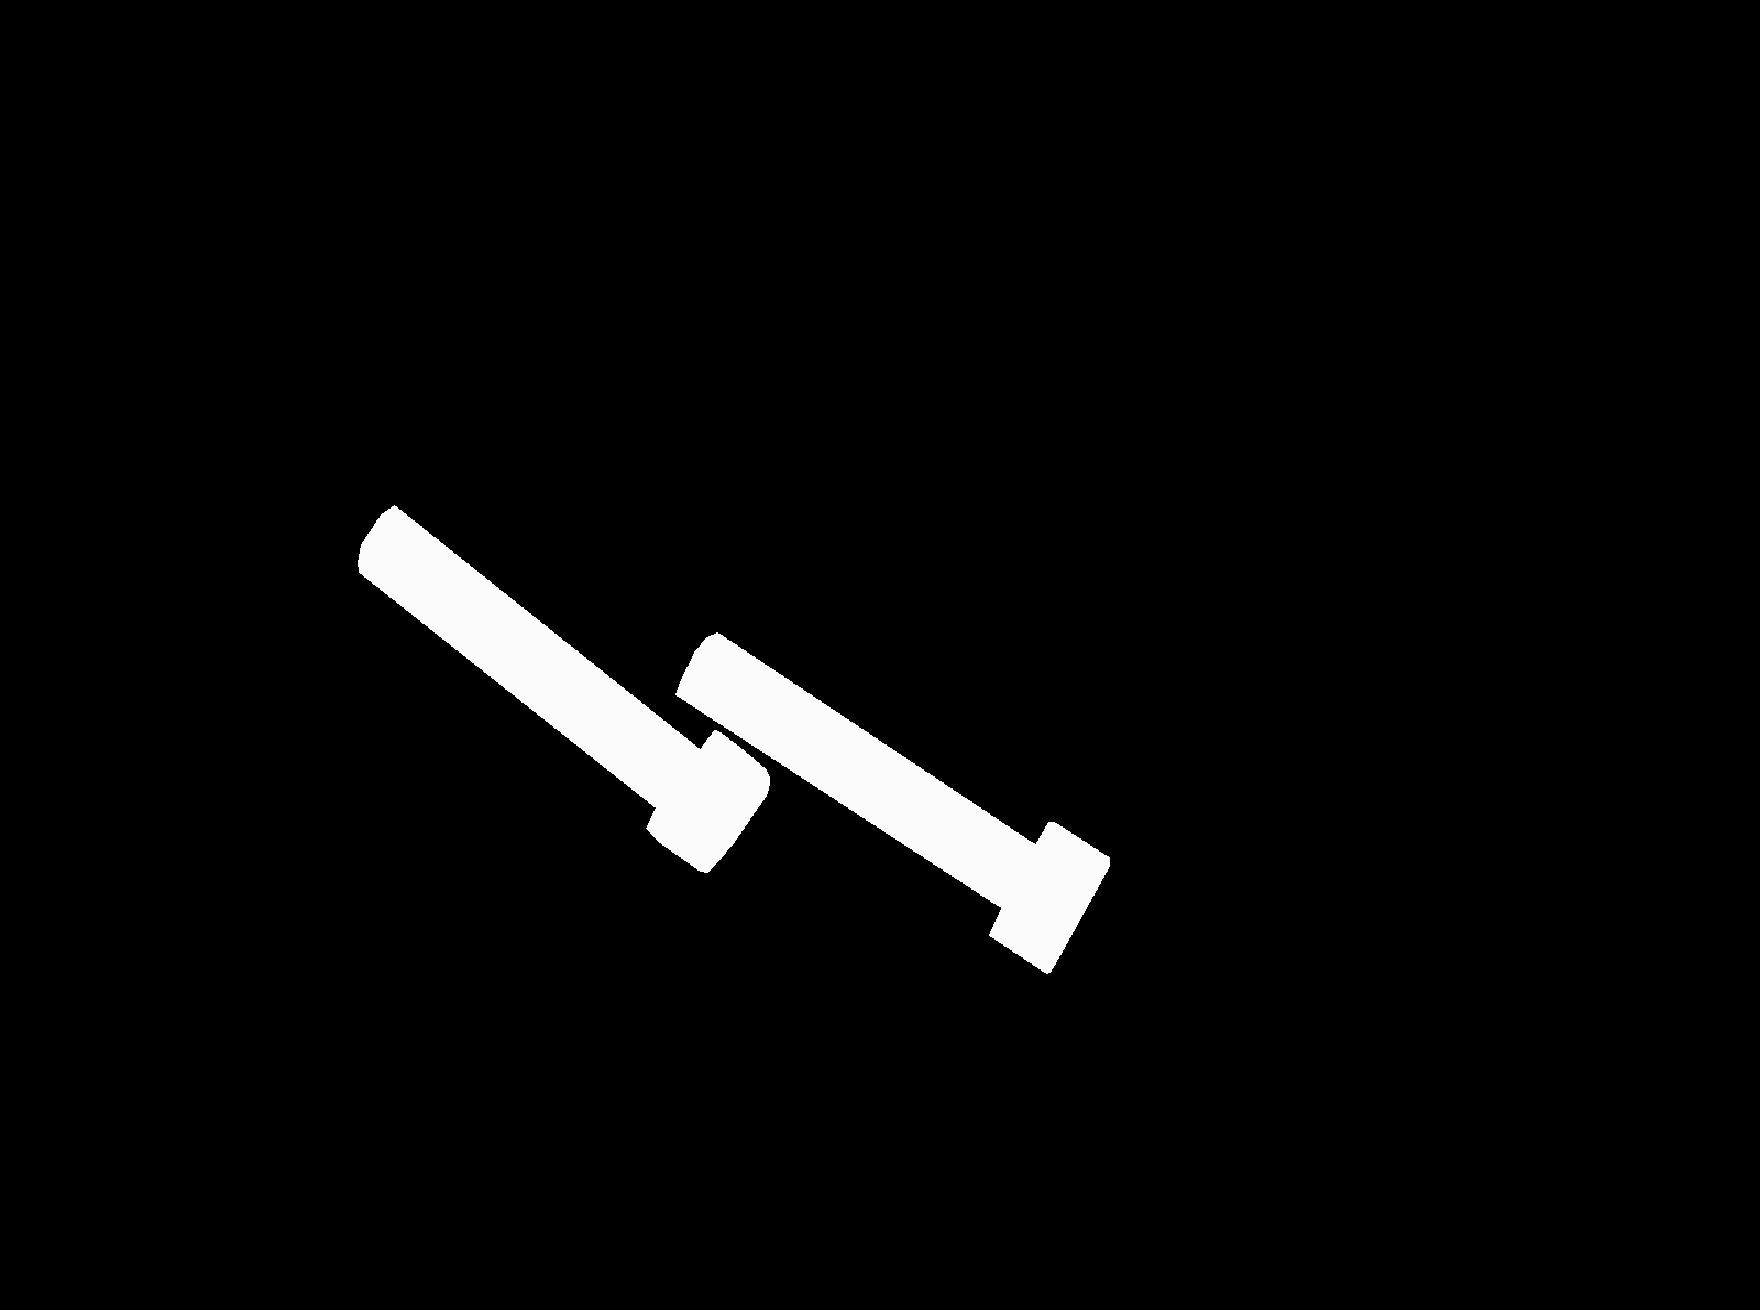
\includegraphics[width=\textwidth]{figures/DRAEMweakness/logical042mask.png}
        \end{minipage}
        \begin{minipage}{0.32\textwidth}
            \centering
            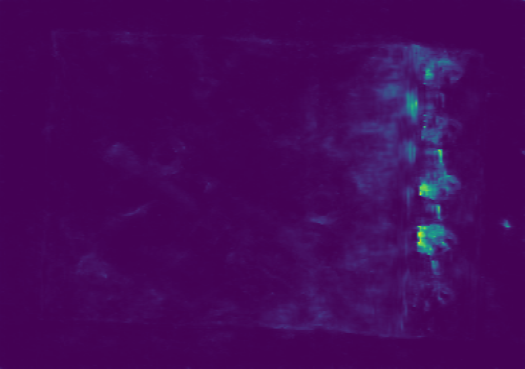
\includegraphics[width=\textwidth]{figures/DRAEMweakness/logical042segment.png}
        \end{minipage}
        \caption{Subfigure 2}
    \end{subfigure}
    \caption{Resulting segmentations of ensemble network training when utilizing layer 4.}
    \label{fig:DRAEMweakness}
\end{figure}